\chapter{Architettura della data pipeline}

\section{Il paradigma della medallion architecture}
Nel trattamento di serie temporali complesse, l'adozione di un'architettura dati strutturata risulta indispensabile per assicurare la tracciabilità delle trasformazioni, l'integrità dei valori e la riproducibilità degli esperimenti. Nel presente progetto è stata implementata la \textbf{Medallion Architecture}, un pattern architetturale ampiamente diffuso nell'ingegneria dei \textbf{data lakehouse} che organizza il flusso di elaborazione in tre stadi logici a qualità progressivamente crescente, denominati convenzionalmente \textbf{Bronze}, \textbf{Silver} e \textbf{Gold}.

Come illustrato nella Figura~\ref{fig:medallion_architecture}, ciascun livello assolve a un compito ben definito all'interno della catena di raffinamento del dato:
il livello \textbf{Bronze} accoglie i dati grezzi estratti direttamente dalla sorgente clinica, salvaguardandoli nella loro forma originaria senza alcuna alterazione;
il livello \textbf{Silver} applica algoritmi di bonifica, normalizzazione, filtraggio degli artefatti sensoristici e partizionamento tematico per reparto;
il livello \textbf{Gold} struttura i dati in documenti conformi al modello a serie storiche di MongoDB, predisponendoli al consumo efficiente da parte delle interfacce grafiche, dei servizi REST e dei modelli di \textbf{machine learning}.

\begin{figure}[ht]
    \centering
    % Diagramma TikZ per la Medallion Architecture (Bronze -> Silver -> Gold)
\begin{tikzpicture}[
    scale=0.92, transform shape,
    font=\sffamily,
    layerBlock/.style={
        draw=brandBorder,
        fill=white,
        rounded corners=8pt,
        line width=1.1pt,
        inner sep=0pt,
        drop shadow={opacity=0.12, shadow xshift=2pt, shadow yshift=-2pt}
    },
    downArrow/.style={
        -{Stealth[length=3.5mm, width=2.5mm]},
        line width=2.2pt,
        color=brandCyan
    }
]

% ==================== LIVELLO 1: LAYER BRONZE ====================
\node[layerBlock, minimum width=15.2cm, minimum height=2.4cm] (bronze) at (0, 4.2) {};

% Barra laterale colorata Bronze
\fill[orange!90!black, rounded corners=7pt] (-7.6, 3.0) rectangle (-7.2, 5.4);

% Intestazione Bronze
\node[anchor=north west] at (-7.0, 5.25) {
    \textbf{\large\color{orange!90!black}LAYER BRONZE} \quad
    \textbf{\normalsize\color{brandNavy}Dati grezzi immutabili} \quad
    \tikz[baseline=-2pt]\node[fill=orange!15, draw=orange!70!black, rounded corners=3pt, font=\scriptsize\bfseries, text=orange!90!black, inner sep=2.5pt]{3.88 MB (100\%)};
};

% Contenuto a 3 colonne Bronze
\node[anchor=north west, font=\footnotesize, align=left] at (-7.0, 4.45) {
    \textbf{\color{brandNavy}Sorgente clinica}\\[2pt]
    \textbullet~VitalDB Open Dataset (API)\\
    \textbullet~5 segnali monitor Solar8000
};

\node[anchor=north west, font=\footnotesize, align=left] at (-1.8, 4.45) {
    \textbf{\color{brandNavy}Formato di storage}\\[2pt]
    \textbullet~Apache Parquet grezzo\\
    \textbullet~Risoluzione nominale 1 secondo
};

\node[anchor=north west, font=\footnotesize, align=left] at (3.2, 4.45) {
    \textbf{\color{brandNavy}Data governance}\\[2pt]
    \textbullet~Immutabilità sorgente assoluta\\
    \textbullet~Registro \texttt{download\_manifest.json}
};


% ==================== TRANSIZIONE 1: CLEAN ====================
\draw[downArrow] (0, 3.0) -- (0, 1.8);
\node[fill=brandSurface, draw=brandCyan, line width=0.9pt, rounded corners=4pt, inner sep=3.5pt, font=\scriptsize\bfseries, text=brandNavy] at (0, 2.4) {
    \texttt{clean.py}: bonifica, filtro range clinici, interpolazione lineare e LOCF
};


% ==================== LIVELLO 2: LAYER SILVER ====================
\node[layerBlock, minimum width=15.2cm, minimum height=2.4cm] (silver) at (0, 0.6) {};

% Barra laterale colorata Silver
\fill[blue!75!cyan, rounded corners=7pt] (-7.6, -0.6) rectangle (-7.2, 1.8);

% Intestazione Silver
\node[anchor=north west] at (-7.0, 1.65) {
    \textbf{\large\color{blue!75!cyan}LAYER SILVER} \quad
    \textbf{\normalsize\color{brandNavy}Bonifica e partizionamento} \quad
    \tikz[baseline=-2pt]\node[fill=blue!12, draw=blue!60!cyan, rounded corners=3pt, font=\scriptsize\bfseries, text=blue!80!black, inner sep=2.5pt]{2.24 MB (-42.4\%)};
};

% Contenuto a 3 colonne Silver
\node[anchor=north west, font=\footnotesize, align=left] at (-7.0, 0.85) {
    \textbf{\color{brandNavy}Pulizia e rimozione}\\[2pt]
    \textbullet~Drop righe senza segnale\\
    \textbullet~Report \texttt{quality\_report.json}
};

\node[anchor=north west, font=\footnotesize, align=left] at (-1.8, 0.85) {
    \textbf{\color{brandNavy}Imputazione temporale}\\[2pt]
    \textbullet~Interp. lineare HR/SpO2 ($\le 5$s)\\
    \textbullet~LOCF NIBP ($\le 300$s) + \texttt{nibp\_age\_s}
};

\node[anchor=north west, font=\footnotesize, align=left] at (3.2, 0.85) {
    \textbf{\color{brandNavy}Partizionamento}\\[2pt]
    \textbullet~Directory \texttt{department=<N>/}\\
    \textbullet~Lettura rapida con pruning
};


% ==================== TRANSIZIONE 2: LOAD ====================
\draw[downArrow] (0, -0.6) -- (0, -1.8);
\node[fill=brandSurface, draw=brandCyan, line width=0.9pt, rounded corners=4pt, inner sep=3.5pt, font=\scriptsize\bfseries, text=brandNavy] at (0, -1.2) {
    \texttt{load\_mongo.py}: modellazione BSON, contratti schema e ingestione time series
};


% ==================== LIVELLO 3: LAYER GOLD ====================
\node[layerBlock, minimum width=15.2cm, minimum height=2.4cm] (gold) at (0, -3.0) {};

% Barra laterale colorata Gold
\fill[brandEmerald, rounded corners=7pt] (-7.6, -4.2) rectangle (-7.2, -1.8);

% Intestazione Gold
\node[anchor=north west] at (-7.0, -1.95) {
    \textbf{\large\color{brandEmerald!90!black}LAYER GOLD} \quad
    \textbf{\normalsize\color{brandNavy}MongoDB Time Series nativo} \quad
    \tikz[baseline=-2pt]\node[fill=brandEmerald!15, draw=brandEmerald, rounded corners=3pt, font=\scriptsize\bfseries, text=brandEmerald!80!black, inner sep=2.5pt]{\textbf{0.42 MB (-89.1\%, 3.7$\times$ speedup)}};
};

% Contenuto a 3 colonne Gold
\node[anchor=north west, font=\footnotesize, align=left] at (-7.0, -2.75) {
    \textbf{\color{brandNavy}Time Series Collection}\\[2pt]
    \textbullet~Collezione \texttt{vital\_signals}\\
    \textbullet~Partizionamento a bucket (1s)
};

\node[anchor=north west, font=\footnotesize, align=left] at (-1.8, -2.75) {
    \textbf{\color{brandNavy}Compressione avanzata}\\[2pt]
    \textbullet~Delta-of-Delta sui timestamp\\
    \textbullet~Zstandard sui vettori biometrici
};

\node[anchor=north west, font=\footnotesize, align=left] at (3.2, -2.75) {
    \textbf{\color{brandNavy}Governance e servizi}\\[2pt]
    \textbullet~Collezioni \texttt{registry} e \texttt{track\_metadata}\\
    \textbullet~Alimentazione API e modelli ML
};

\end{tikzpicture}

    \caption{Panoramica dell'architettura Medallion e dei livelli Bronze, Silver e Gold generata in TikZ.}
    \label{fig:medallion_architecture}
\end{figure}

L'adozione di questa architettura multi-stadio garantisce che gli errori introdotti in un passaggio intermedio possano essere isolati e corretti rieseguendo le trasformazioni a partire dai livelli precedenti, preservando al contempo una netta separazione delle responsabilità tra ingestione, trasformazione analitica e fruizione finale del dato.

L'intera catena di elaborazione, schematizzata nella Figura~\ref{fig:pipeline_execution}, si articola in cinque fasi operative sequenziali che connettono l'estrazione remota alla visualizzazione telemetrica.

\begin{figure}[ht]
    \centering
    \resizebox{0.95\textwidth}{!}{% === DIAGRAMMA PIPELINE DI ESECUZIONE END-TO-END (LAYOUT HORSESHOE PERFETTO) ===
\begin{tikzpicture}[
    font=\sffamily,
    >=Stealth,
    stage/.style={
        rectangle,
        rounded corners=7pt,
        draw=brandBorder,
        line width=1.1pt,
        fill=white,
        drop shadow={opacity=0.07, shadow xshift=1.5pt, shadow yshift=-2pt},
        inner sep=8pt,
        align=center
    },
    bronzeBox/.style={stage, draw=brandCoral!65, fill=brandPeach!10},
    silverBox/.style={stage, draw=brandPrimary!60, fill=brandPrimary!6},
    goldBox/.style={stage, draw=brandTeal!60, fill=brandTeal!8},
    detectBox/.style={stage, draw=brandPrimary!75, fill=brandPrimary!5},
    serveBox/.style={stage, draw=brandDark!60, fill=brandSurface},
    flowArrow/.style={
        ->,
        line width=1.6pt,
        color=brandPrimary
    }
]

% ================= RIGA 1: DATA PIPELINE (SINISTRA -> DESTRA) =================
% FASE 1: BRONZE
\node[bronzeBox, text width=3.8cm] (p1) {
    {\sffamily\bfseries\scriptsize\textcolor{brandNavy}{FASE 1: BRONZE}}\\[3pt]
    \textbf{\footnotesize Ingestione Grezza}\\[2pt]
    {\scriptsize
    $\bullet$ VitalDB Public API\\
    $\bullet$ 50 casi clinici chirurgia\\
    $\bullet$ Parquet raw senza schema\\
    $\bullet$ 3.88 MB / 644.637 record
    }
};

% FASE 2: SILVER
\node[silverBox, text width=4.2cm, right=2.2cm of p1] (p2) {
    {\sffamily\bfseries\scriptsize\textcolor{brandBlue}{FASE 2: SILVER}}\\[3pt]
    \textbf{\footnotesize Bonifica \& Partizionamento}\\[2pt]
    {\scriptsize
    $\bullet$ Bounding fisiologico\\
    $\bullet$ Drop righe prive di segnale\\
    $\bullet$ Interpolazione lineare $\le 5$s\\
    $\bullet$ LOCF NIBP $\le 300$s\\
    $\bullet$ Calcolo metadato \texttt{nibp\_age\_s}\\
    $\bullet$ Partizionamento Hive Parquet
    }
};

% FASE 3: GOLD
\node[goldBox, text width=4.1cm, right=2.2cm of p2] (p3) {
    {\sffamily\bfseries\scriptsize\textcolor{brandCyan!85!black}{FASE 3: GOLD}}\\[3pt]
    \textbf{\footnotesize MongoDB Time Series}\\[2pt]
    {\scriptsize
    $\bullet$ Collezione \texttt{vital\_signals}\\
    $\bullet$ Compressione bucket nativa\\
    $\bullet$ Delta-of-Delta a 1 Hz\\
    $\bullet$ Metastore catalogo \texttt{registry}\\
    $\bullet$ JSON Schema rigoroso\\
    $\bullet$ Omissione campi nulli BSON
    }
};

% ================= RIGA 2: DETECTION & SERVING (DESTRA -> SINISTRA) =================
% FASE 4: ANOMALY DETECTION (posizionata verticalmente sotto FASE 3: GOLD)
\node[detectBox, text width=6.6cm, below=2.0cm of p3] (p4) {
    {\sffamily\bfseries\scriptsize\textcolor{brandPrimary}{FASE 4: ANOMALY DETECTION MULTILIVELLO}}\\[3pt]
    \textbf{\footnotesize Inferenza Ibrida (\texttt{POST /detect})}\\[4pt]
    \begin{tabular}{@{}p{3.0cm}@{\hspace{8pt}}p{3.0cm}@{}}
        \centering
        \textbf{\tiny REGOLE CLINICHE}\\[2pt]
        {\tiny
        $\bullet$ Shock Index $> 0.9$\\
        $\bullet$ Ipotensione severa\\
        ($MBP < 65 \land \text{SpO}_2 < 90\%$)
        }
        &
        \centering
        \textbf{\tiny MACHINE LEARNING}\\[2pt]
        {\tiny
        $\bullet$ Isolation Forest (5\%)\\
        $\bullet$ LSTM Autoencoder\\
        $\bullet$ Errore $\max_c \text{MSE}_c$ al 95° pct
        }
    \end{tabular}\\[4pt]
    {\scriptsize $\Downarrow$ Persistenza atomica in \texttt{anomalies\_detected}}
};

% FASE 5: SERVING & DASHBOARD (posizionata alla sinistra di FASE 4, sotto FASE 1 e 2)
\node[serveBox, text width=7.0cm, left=2.5cm of p4] (p5) {
    {\sffamily\bfseries\scriptsize\textcolor{brandNavy}{FASE 5: SERVING \& DASHBOARD}}\\[3pt]
    \textbf{\footnotesize Fruizione Dati \& Visualizzazione Telemetrica}\\[3pt]
    {\scriptsize
    $\bullet$ Downsampling analitico con pipeline MongoDB \texttt{\$dateTrunc}\\
    $\bullet$ Server ASGI asincrono FastAPI con pool di connessione PyMongo\\
    $\bullet$ Frontend modulare a componenti con loader asincrono HTML\\
    $\bullet$ Consensus Matrix multimodello con modali clinici ed esplicativi\\
    $\bullet$ Grafici telemetrici sincronizzati (HR, $\text{SpO}_2$, SBP, DBP, MBP)
    }
};

% ================= FRECCE DI FLUSSO CON ETICHETTE PULITE =================
% Flusso orizzontale superiore (Bronze -> Silver -> Gold)
\draw[flowArrow] (p1.east) -- node[above=4pt, font=\scriptsize\bfseries, text=brandCyan!85!brandNavy, align=center] {Bonifica \&\\Imputazione} (p2.west);
\draw[flowArrow] (p2.east) -- node[above=4pt, font=\scriptsize\bfseries, text=brandCyan!85!brandNavy, align=center] {Caricamento\\\texttt{load\_mongo.py}} (p3.west);

% Transizione verticale lineare diretta (Gold -> Detection)
\draw[flowArrow] (p3.south) -- node[right=6pt, font=\scriptsize\bfseries, text=brandTeal!85!black, align=left] {Estrazione serie\\per paziente} (p4.north);

% Flusso orizzontale inferiore di consumo (Detection -> Serving)
\draw[flowArrow] (p4.west) -- node[above=4pt, font=\scriptsize\bfseries, text=brandNavy, align=center] {Allarmi rilevati \&\\downsampling} (p5.east);

\end{tikzpicture}
}
    \caption{Architettura della pipeline di esecuzione end-to-end dall'ingestione alla visualizzazione.}
    \label{fig:pipeline_execution}
\end{figure}

\section{Layer Bronze per l'ingestione e la storicizzazione dei dati grezzi}
Il livello \textbf{Bronze} costituisce il punto di ingresso dell'intera infrastruttura. Il modulo di acquisizione, implementato nello script \texttt{src/bronze/download.py}, interagisce direttamente con l'archivio centrale di VitalDB sfruttando l'API Python ufficiale.

L'ingestione seleziona in modo automatico i casi clinici tramite la funzione \texttt{vitaldb.find\_cases}, che individua i pazienti per i quali risultano registrate contemporaneamente le cinque metriche fisiologiche di interesse: la frequenza cardiaca, la saturazione d'ossigeno e le tre componenti pressorie. Per ciascun caso individuato, la procedura scarica i tracciati temporali mediante \texttt{vitaldb.load\_case} impostando una frequenza nominale di campionamento pari a un secondo (\texttt{interval=1.0}).

I tracciati acquisiti vengono persistiti in locale nella cartella \texttt{data/bronze/} all'interno di file conformi allo standard Apache Parquet, con convenzione di denominazione \texttt{case\_<ID>.parquet}. La scelta del formato Parquet per lo strato grezzo rispetto al testo semplice CSV è motivata dalla natura colonnare e compressa del formato, che riduce in misura rilevante lo spazio occupato su disco e memorizza in modo nativo i tipi di dato numerici a virgola mobile a 64 bit, scongiurando qualsiasi perdita di precisione numerica o ambiguità di codifica.

Contestualmente all'acquisizione dei segnali temporali, la procedura estrae le informazioni cliniche e perioperatorie salvandole nel file ausiliario \texttt{data/bronze/clinical\_data.parquet}, che raccoglie attributi fondamentali quali l'età del paziente, il sesso, l'indice di massa corporea e il reparto chirurgico di ricovero. Poiché l'implementazione predefinita della funzione \texttt{vitaldb.load\_clinical\_data()} nella libreria Python ufficiale presenta un noto difetto che restituisce una tabella vuota se invocata senza argomenti espliciti, il modulo \texttt{download.py} interroga in via prioritaria l'endpoint REST ufficiale (\texttt{https://api.vitaldb.net/cases}), mantenendo l'SDK parametrizzato come meccanismo di fallback. Qualora entrambe le modalità dovessero fallire o restituire zero record, la pipeline applica una politica \textbf{fail-fast} interrompendo immediatamente l'esecuzione con codice di uscita non nullo (\texttt{sys.exit(1)}): questo blocco preventivo è motivato dal fatto che un'ingestione priva della mappatura dei reparti chirurgici degraderebbe silenziosamente l'intero partizionamento del successivo livello \textbf{Silver}, riversando tutti i pazienti nella partizione residuale \texttt{department=UNKNOWN}. A completamento del contesto clinico, la funzione \texttt{download\_lab\_data} scarica e filtra sui soli \texttt{case\_id} della coorte anche i referti ematochimici perioperatori, persistendoli in \texttt{data/bronze/lab\_data.parquet}.

In conformità con i principi di \textbf{data governance}, il livello \textbf{Bronze} adotta una politica di immutabilità rigorosa: i file vengono memorizzati esattamente nello stato in cui sono stati emessi dalla sorgente remota, senza alcuna rimozione di valori nulli o alterazione temporale. Per garantire una tracciabilità formale (\textbf{data lineage}) lungo l'intera catena, l'avvio dello script \texttt{download.py} genera un identificativo univoco di esecuzione (\texttt{run\_id}, persistito in \texttt{data/.current\_run\_id} tramite \texttt{config.get\_or\_create\_run\_id}) che viene inciso, insieme alla versione della pipeline (\texttt{pipeline\_version = "1.1.0"}), all'interno del registro strutturato \texttt{download\_manifest.json}. Tale manifest censisce per ogni singolo caso l'esito puntuale (\texttt{downloaded}, \texttt{skipped\_existing} o \texttt{failed}), il numero di campioni e il peso in byte. Inoltre, prima di saltare il download di un file Parquet già presente su disco (\texttt{skipped\_existing}), la funzione \texttt{download\_case} ispeziona la struttura del file per verificare che contenga effettivamente tutte le cinque tracce richieste più la colonna \texttt{Time} e che il passo di campionamento coincida con \texttt{SAMPLING\_INTERVAL} ($1.0\text{ s}$): questa verifica impedisce che file residui generati da esecuzioni precedenti con configurazioni o frequenze differenti inquinino silenziosamente la corsa corrente.

\section{Layer Silver per la bonifica e il partizionamento dei dati}
I dati clinici immagazzinati nel livello \textbf{Bronze} non possono essere impiegati direttamente per l'addestramento di modelli predittivi o per il monitoraggio in tempo reale a causa della notevole quantità di rumore, discontinuità e valori nulli. Il livello \textbf{Silver}, orchestrato dallo script \texttt{src/silver/clean.py}, si fa carico della bonifica del dato, della gestione dei valori mancanti, dell'etichettatura degli outlier fisiologici, del tracciamento esplicito delle imputazioni per singolo canale e della riorganizzazione fisica dei file su file system. Prima di avviare l'elaborazione, la funzione \texttt{process\_all\_cases} riallinea automaticamente il perimetro dei casi rispetto al \texttt{download\_manifest.json} attivo (o al limite configurato \texttt{MAX\_CASES = 500}), rimuovendo eventuali file Parquet \textbf{Silver} orfani di esecuzioni precedenti con perimetro differente, così da garantire che tutti i layer descrivano esattamente la medesima coorte.

Un requisito metodologico fondamentale nella pulizia di serie temporali a $1\text{ Hz}$ consiste nel preservare l'integrità della griglia temporale durante le operazioni di interpolazione. Se si eliminassero in apertura le righe completamente vuote (\texttt{dropna(how='all')}), due campioni originariamente separati da un'interruzione di molti minuti diverrebbero artificialmente adiacenti nell'indice del DataFrame, falsando il significato fisico delle finestre temporali espresse in numero di campioni. Per questa ragione, nel modulo \texttt{clean.py} la griglia temporale a $1\text{ Hz}$ viene mantenuta intatta durante tutte le fasi di controllo e imputazione, posticipando lo scarto delle righe prive di qualsiasi misurazione su tutte e cinque le tracce (5.565.384 campioni grezzi ridotti a 5.402.386 secondi attivi, con 162.998 righe vuote rimosse ai margini dell'intervento) esclusivamente al termine del flusso di pulizia.

La prima trasformazione eseguita sulla griglia integra consiste nell'identificazione degli outlier fisiologici \textbf{prima} di qualsiasi operazione di interpolazione o trascinamento in avanti. Per eliminare il rischio di divergenze tra i moduli Python di pulizia e gli schemi di catalogo del database, i limiti fisiologici di plausibilità sono stati centralizzati in un'unica fonte di verità (\textbf{Single Source of Truth}), rappresentata dal dizionario \texttt{TRACK\_SPECS} nel modulo \texttt{src/config.py}:
frequenza cardiaca considerata valida tra $20$ e $250$ bpm;
saturazione periferica considerata valida tra il $50\%$ e il $100\%$;
pressione sistolica considerata valida tra $40$ e $250$ mmHg;
pressione diastolica considerata valida tra $10$ e $180$ mmHg (uniformando il limite superiore tra codice di pulizia e catalogo metadati);
pressione media considerata valida tra $20$ e $220$ mmHg.

I valori osservati che cadono al di fuori di questi intervalli non vengono cancellati distruttivamente dalla riga originale, bensì etichettati tramite cinque flag booleani dedicati (\texttt{HR\_outlier}, \texttt{SPO2\_outlier}, \texttt{SBP\_outlier}, \texttt{DBP\_outlier}, \texttt{MBP\_outlier}). Calcolare questi flag sui dati grezzi prima dell'imputazione — e mascherare temporaneamente gli outlier durante il calcolo dell'interpolazione e del forward-fill — risponde a una precisa motivazione clinica e statistica: se gli outlier venissero valutati dopo il trascinamento LOCF, una singola lettura pressoria aberrante causata dalla compressione accidentale del bracciale da parte del chirurgo verrebbe propagata in avanti per i successivi 300 secondi, trasformando un artefatto puntuale di un secondo in 301 secondi consecutivi di falsi outlier e corrompendo le statistiche di qualità.

Successivamente, il modulo applica una strategia differenziata di imputazione (con tracciamento esplicito tramite flag booleani \texttt{*\_imputed} per ciascuno dei cinque canali) per gestire la disomogeneità fisiologica delle sorgenti sensoristiche:
per i segnali fisiologici continui, segnatamente la frequenza cardiaca (\texttt{Solar8000/HR}) e la saturazione periferica (\texttt{Solar8000/PLETH\_SPO2}), le brevi perdite di segnale causate da artefatti di movimento vengono sanate mediante la funzione dedicata \texttt{interpolate\_short\_gaps(series, max\_gap=5)}:
$$y(t) = y(t_0) + \frac{y(t_1) - y(t_0)}{t_1 - t_0} (t - t_0)$$
A differenza del metodo standard \texttt{.interpolate(limit=5)} della libreria \texttt{pandas} — che riempie indiscriminatamente i primi cinque campioni anche all'inizio di un'interruzione strumentale lunga diversi minuti, generando "code" sintetiche prive di significato biologico — la funzione \texttt{interpolate\_short\_gaps} calcola preliminarmente l'ampiezza complessiva di ciascun blocco contiguo di valori mancanti e applica l'interpolazione lineare \textbf{esclusivamente} ai buchi interni di durata totale $\le 5\text{ s}$ compresi tra due misure valide. Le interruzioni di durata superiore a cinque secondi e i valori mancanti periferici vengono lasciati intatti a \texttt{NaN}, mentre i punti effettivamente ricostruiti vengono marcati nei flag booleani \texttt{HR\_imputed} e \texttt{SPO2\_imputed};
per i segnali pressori non invasivi (\texttt{NIBP\_SBP}, \texttt{NIBP\_DBP}, \texttt{NIBP\_MBP}), la misurazione è intrinsecamente intermittente, avvenendo a intervalli discreti compresi tipicamente tra due e cinque minuti mediante il ciclo oscillometrico del bracciale. In questo scenario viene adottata la tecnica \textbf{Last Observation Carried Forward} (LOCF), propagando l'ultimo valore valido non-outlier:
$$y(t) = y(t_{\text{last}}) \quad \forall t \in [t_{\text{last}}, t_{\text{last}} + 300\text{ s}]$$
La propagazione è limitata a una finestra massima di 300 secondi (cinque minuti) e viene tracciata individualmente per ciascuna componente pressoria tramite le colonne booleane \texttt{SBP\_imputed}, \texttt{DBP\_imputed} e \texttt{MBP\_imputed}. Tracciare separatamente le tre componenti (anziché dedurre il numero di imputazioni indirettamente dalla sola età del bracciale) garantisce conteggi di qualità esatti anche nei rari istanti in cui il monitor restituisce una lettura parziale.

A supporto della trasparenza analitica, dell'auditing clinico e del filtraggio a valle nelle regole diagnostiche, il modulo calcola contestualmente la variabile temporale \texttt{nibp\_age\_s}:
$$\texttt{nibp\_age\_s} = t - t_{\text{last\_cuff}}$$
Tale grandezza quantifica in ogni secondo l'età dell'ultima misurazione pressoria valida registrata su almeno un canale del bracciale. Questo metadato si rivela determinante sia per il clinico sia per il motore di \textbf{anomaly detection}: come vedremo nel Capitolo 4, le regole cliniche interrogano direttamente \texttt{nibp\_age\_s} per inibire l'emissione di allarmi emodinamici qualora la pressione propagata per LOCF abbia superato la soglia di freschezza clinica di 120 secondi.

\begin{figure}[ht]
    \centering
    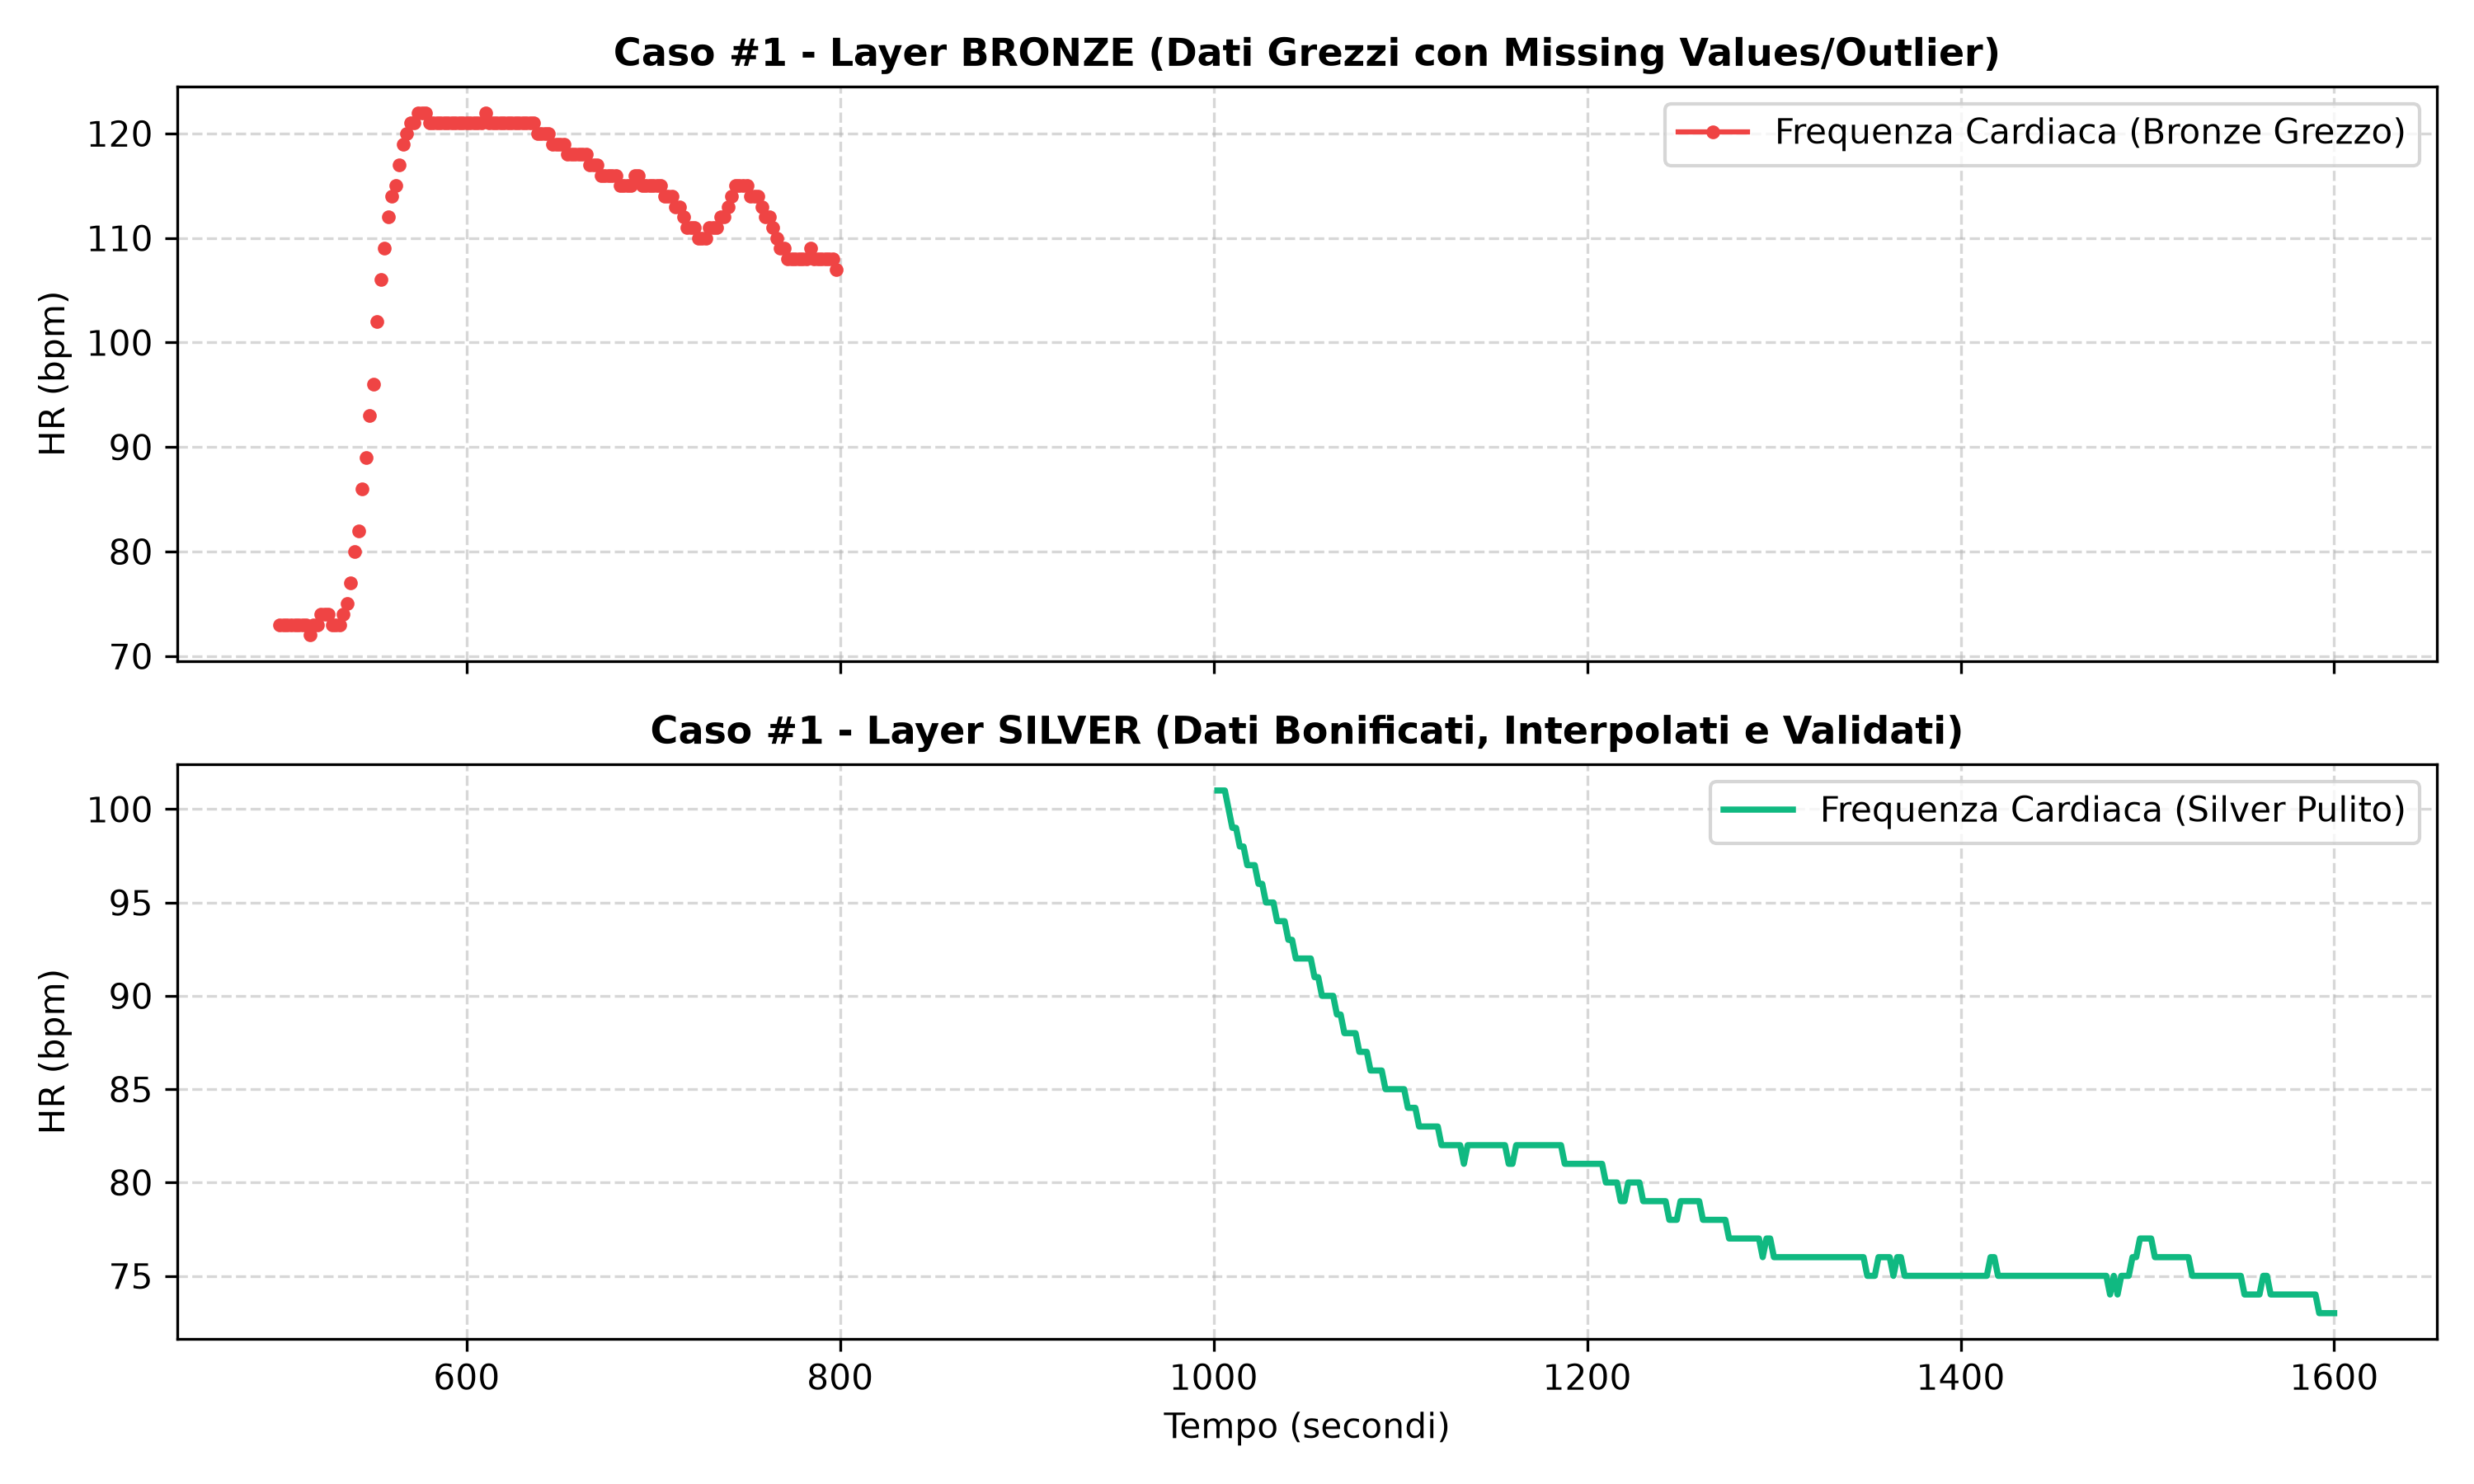
\includegraphics[width=0.88\textwidth]{before_after_cleaning.png}
    \caption{Confronto visivo tra il tracciato della frequenza cardiaca grezzo (Bronze) e bonificato (Silver).}
    \label{fig:before_after}
\end{figure}

La Figura~\ref{fig:before_after} mette a confronto l'andamento del tracciato della frequenza cardiaca di un paziente reale prima e dopo l'intervento di bonifica. Nella parte superiore, il segnale grezzo estratto dal livello \textbf{Bronze} presenta evidenti salti e interruzioni causati da temporanee perdite di aderenza del sensore; nella parte inferiore, il segnale pulito del livello \textbf{Silver} si presenta continuo nei micro-gap fisiologici ma fedele alle reali interruzioni prolungate.

L'implementazione concreta di queste trasformazioni è descritta nel Listato~\ref{lst:clean_imputation}, estratto dal modulo \texttt{src/silver/clean.py}.

\begin{lstlisting}[caption={Algoritmo di identificazione preventiva degli outlier, interpolazione selettiva dei gap brevi e tracciamento esplicito nel layer Silver.}, label={lst:clean_imputation}]
// Codice estratto da src/silver/clean.py
# 1. Identifica gli outlier fisiologici SUI DATI GREZZI (da config.TRACK_SPECS) prima dell'imputazione
for track_name, flag_col in outlier_map.items():
    spec = config.TRACK_SPECS.get(track_name, {})
    val = df_clean[track_name]
    df_clean[flag_col] = val.notna() & ((val < spec["min"]) | (val > spec["max"]))

# 2. Segnali continui (HR e SpO2): interpola solo buchi interni <= 5s senza propagare outlier
clean_hr, hr_imp = interpolate_short_gaps(raw_hr.mask(out_hr), max_gap=5)
df_clean['Solar8000/HR'] = clean_hr.where(~out_hr, raw_hr)
df_clean['HR_imputed'] = hr_imp & (~out_hr)

# 3. Segnali NIBP: calcolo nibp_age_s e LOCF individuale (max 300s) senza trascinare outlier
last_measure_time = time_series.where(any_valid_nibp).ffill()
df_clean['nibp_age_s'] = (time_series - last_measure_time).fillna(9999.0).astype(float)
for t, o, imp_col in present_nibp:
    filled_col = df_clean[t].mask(df_clean[o]).ffill(limit=300)
    df_clean[t] = filled_col.where(~df_clean[o], df_clean[t])
    df_clean[imp_col] = was_na & df_clean[t].notna()

# 4. Scarta solo alla fine le righe in cui tutte le tracce vitali sono simultaneamente nulle
df_clean = df_clean.dropna(subset=vital_cols, how='all').copy()
\end{lstlisting}

\begin{techbox}[brandTeal]{Sintesi di data governance nel layer Silver}
L'architettura del layer Silver garantisce che nessun artefatto venga propagato o nascosto: i limiti fisiologici sono letti da un'unica fonte centralizzata (\texttt{TRACK\_SPECS}), gli outlier sono marcati prima dell'imputazione così da non essere trascinati dal forward-fill, l'interpolazione lineare è circoscritta ai soli buchi interni $\le 5\text{ s}$ (\texttt{interpolate\_short\_gaps}), e ciascuno dei 5 canali dispone di un flag booleano dedicato (\texttt{*\_imputed}) oltre al contatore di freschezza $\texttt{nibp\_age\_s}$.
\end{techbox}

Infine, i dati bonificati vengono salvati in formato Parquet all'interno di una gerarchia di directory partizionata fisicamente per reparto chirurgico di appartenenza (\texttt{department}):
$$\texttt{data/silver/department=<REPARTO>/case\_<ID>.parquet}$$
Questa organizzazione ricalca il principio del \textbf{partition pruning} dei moderni \textbf{data lakehouse}: quando un'interrogazione o una procedura di addestramento richiede i dati relativi a una specifica specialità chirurgica, il lettore Apache Parquet ispeziona unicamente il sottoalbero della directory corrispondente senza scansionare l'intero archivio su disco, abbattendo le operazioni di I/O e velocizzando l'elaborazione.

\section{Evoluzione del modello dati da tabella piatta a documento BSON}
L'architettura della pipeline non si limita a innalzare la qualità intrinseca dei valori numerici, ma trasforma radicalmente il modello concettuale del dato nel passaggio verso il livello \textbf{Gold}.

Nei livelli \textbf{Bronze} e \textbf{Silver}, i dati risiedono sotto forma di tabelle piatte bidimensionali all'interno di file Parquet (6 colonne nel \textbf{Bronze}, arricchite a 18 colonne nel \textbf{Silver} per includere i dieci flag booleani di outlier e imputazione, l'età della misura pressoria \texttt{nibp\_age\_s} e l'identificativo \texttt{case\_id}). Questo modello tabulare classico, pur risultando ideale per elaborazioni vettoriali in memoria tramite librerie quali \texttt{pandas}, mostra evidenti limiti nel contesto dell'archiviazione distribuita e del monitoraggio clinico in tempo reale: ogni riga ripete pedissequamente gli identificatori del paziente, alloca colonne booleane anche quando tutti i flag sono falsi e richiede schemi rigidi poco adatti all'evoluzione dei parametri monitorati.

Nel livello \textbf{Gold}, il dato viene rimodellato come documento gerarchico BSON all'interno di MongoDB. La struttura del documento, mostrata nel Listato~\ref{lst:bson_gold}, è articolata in quattro sezioni logiche:
il campo radice \texttt{timestamp}, che definisce l'ordinamento temporale ed è memorizzato come oggetto nativo \texttt{ISODate};
il sotto-documento \texttt{metadata}, che raccoglie in modo compatto tutte le proprietà immutabili del paziente e del sensore, tra cui l'identificativo del caso (\texttt{case\_id}), il nome del monitor sorgente (\texttt{sensor\_name}), il reparto chirurgico, l'età e il sesso;
il sotto-documento \texttt{metrics}, che incapsula i soli valori numerici delle misurazioni fisiologiche effettivamente presenti in quel secondo, opportunamente sanitizzati sostituendo i caratteri di barra con trattini bassi per evitare conflitti con la sintassi a percorsi di MongoDB;
il sotto-documento \texttt{quality\_flags}, che eredita dal livello \textbf{Silver} sia i cinque flag booleani \texttt{*\_outlier} sia i cinque flag \texttt{*\_imputed} e il contatore di freschezza \texttt{nibp\_age\_s}, preservando integralmente la qualifica di affidabilità e provenienza di ciascuna misurazione.

\begin{lstlisting}[caption={Evoluzione del dato dal formato Parquet piatto al documento BSON nel layer Gold.}, label={lst:bson_gold}]
// Documento gerarchico BSON archiviato nella collezione 'vital_signals'
{
  "_id": ObjectId("65d3f1a0e4b01a2b3c4d5e6f"),
  "timestamp": ISODate("2020-01-01T08:15:30Z"),
  "metadata": {
    "case_id": 1,
    "sensor_name": "Solar8000",
    "department": "General surgery",
    "age": 64,
    "sex": "M"
  },
  "metrics": {
    "Solar8000_HR": 72.0,
    "Solar8000_PLETH_SPO2": 98.0,
    "Solar8000_NIBP_SBP": 120.0,
    "Solar8000_NIBP_DBP": 80.0,
    "Solar8000_NIBP_MBP": 93.3
  },
  "quality_flags": {
    "HR_outlier": false, "SPO2_outlier": false,
    "SBP_outlier": false, "DBP_outlier": false, "MBP_outlier": false,
    "HR_imputed": false, "SPO2_imputed": false,
    "SBP_imputed": true, "DBP_imputed": true, "MBP_imputed": true,
    "nibp_age_s": 14.0
  }
}
\end{lstlisting}

Questa rappresentazione semi-strutturata si rivela decisiva per sfruttare appieno le capacità del motore \textbf{Time Series} di MongoDB, poiché isola i metadati descrittivi dal flusso continuo delle metriche numeriche, abilitando strategie avanzate di compressione e indicizzazione.
